\section{Almost-Sure Termination of Sampling Algorithms}
\label{sec:case-studies}

\subsection{Fast Dice Roller: The Same Proof at Two Levels}
\label{sec:fdr}

\subsubsection{Program and Invariant.}

The Fast Dice Roller (FDR) samples uniformly from $\{0,\ldots,n-1\}$ using fair coin flips~\cite{DBLP:journals/corr/abs-1304-1916}. We use the following program-level presentation:
\begin{lstlisting}[basicstyle=\ttfamily\small,mathescape=true,frame=single]
$v := 1;\ c := 0;$
while ($v<n$) do
  $v := 2v;$
  $c := 2c$ [1/2] $c := 2c+1;$
  if ($c\ge n$) then $v:=v-n;\ c:=c-n$ else skip
end
\end{lstlisting}
On termination, $c$ is the sampled outcome. Existing distributional-invariant reasoning proves that the terminating output is uniform~\cite{zilken2026verifyingsamplingalgorithmsdistributional}; AST completes total correctness. The distributional invariant taken from ~\cite{zilken2026verifyingsamplingalgorithmsdistributional} states that at the loop head, the reachable states satisfy
\begin{equation}
 0\le c<\min(v,n),\qquad 0<v<2n,\qquad n>0.
 \label{eq:fdr-support}
\end{equation}
Here $n,v,c$ are integers, as ensured by initialization and preserved by the
body. The distributional invariant additionally states that equal admissible
$c$-values carry equal mass; only its support information
\eqref{eq:fdr-support} and integrality are needed for our termination proof.

\subsubsection{Program-Level AST Proof.}
Let $B_{\mathrm{FDR}}$ denote the body. For bit $\beta\in\{0,1\}$,
write $t_\beta=2c+\beta$ and define the complete update
\[
 F_\beta(\sigma)=
 \begin{cases}
   \sigma[v/2v-n,c/t_\beta-n],&t_\beta\geq n,\\
   \sigma[v/2v,c/t_\beta],&t_\beta<n.
 \end{cases}
\]
All expressions on the right are evaluated in the input state $\sigma$.
The one-iteration post-distribution is therefore
\begin{equation}
 \post{B_{\mathrm{FDR}}}(\dirac{\sigma})
 =\tfrac12\dirac{F_0(\sigma)}+\tfrac12\dirac{F_1(\sigma)}.
 \label{eq:fdr-post}
\end{equation}
This calculation includes the conditional recycling after either bit.

\paragraph{Motivation: shortest paths to termination.}
Consider the iteration-level Markov chain: its states are loop-head states,
and each transition from an enabled state summarizes one complete execution
of $B_{\mathrm{FDR}}$, including possible recycling. States with $v\geq n$
are terminal. Let $d_{\min}(\sigma)$ be the length of a shortest
positive-probability path from $\sigma$ to a terminal state, measured in
\emph{complete loop iterations}; terminal states have distance zero.

To obtain a simple bound on this distance, write $\Delta=v-c$. In an
enabled state, \eqref{eq:fdr-support} gives $1\leq\Delta\leq n-1$.
Choosing bit zero doubles $\Delta$, and subtracting $n$ from both variables
preserves their difference. Consequently, after
\[
 k=\left\lceil\log_2\!\left(\frac{n}{v-c}\right)\right\rceil
\]
consecutive zero bits, either the loop has already terminated or its
difference would be $2^k\Delta\geq n$, which is impossible at an enabled
loop head. Such a bit sequence has positive probability. Thus every
enabled state has a finite shortest distance satisfying
\begin{equation}
 d_{\min}(\sigma)\leq
 \left\lceil\log_2\!\left(\frac{n}{v-c}\right)\right\rceil.
 \label{eq:fdr-shortest-distance-bound}
\end{equation}
This shortest-path view, following Seidel~\cite[Section~5.3]{seidel2026thesis},
motivates our logarithmic variant below. The bound
need not be exact: for $n=6$ and $(v,c)=(4,2)$ it equals $2$, although both
successors, $(8,4)$ and $(8,5)$, are terminal, so $d_{\min}=1$.
\Cref{fig:fdr-iteration-variants} contrasts the two functions.

% The iteration-level presentation is inspired by Figure 5.2 of
% Jonas Seidel's Master's thesis (2026), DOI: 10.18154/RWTH-2026-04488.
% This new drawing contracts all recycling updates and shows actual
% shortest distances alongside the terminal-normalized logarithmic variant.
\begin{figure}[t]
 \centering
 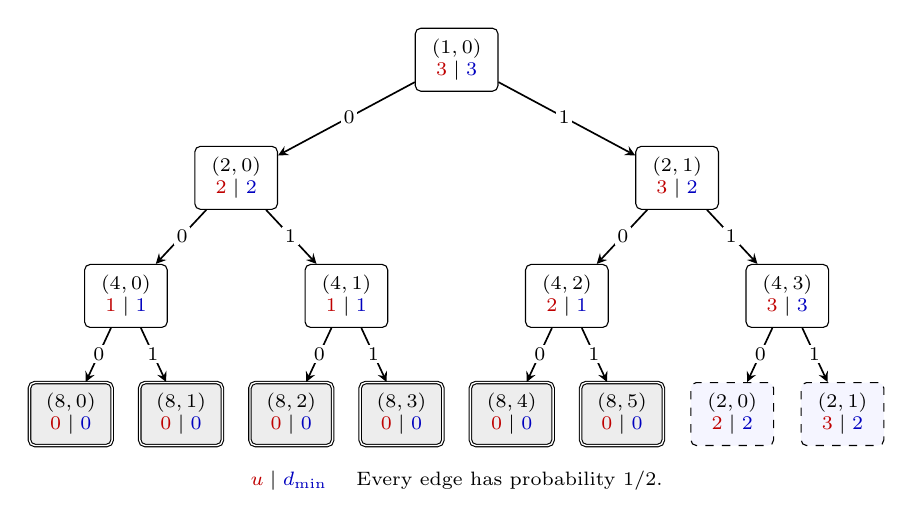
\begin{tikzpicture}[
   x=1.4cm,y=1cm,>=stealth,
   fdrstate/.style={draw,rounded corners=2pt,minimum width=10.5mm,
     minimum height=8mm,inner sep=2pt,align=center,font=\scriptsize},
   fdrterminal/.style={fdrstate,fill=black!7,double,double distance=0.5pt},
   fdrrecycled/.style={fdrstate,dashed,fill=blue!4},
   fdrbit/.style={font=\scriptsize,fill=white,inner sep=1pt},
   fdredge/.style={->,semithick}
 ]
 % Each node displays (v,c), then u | d_min.
 \node[fdrstate] (s10) at (3.5,4.5)
   {$(1,0)$\\$\textcolor{red!75!black}{3}\mid\textcolor{blue!75!black}{3}$};
 \node[fdrstate] (s20) at (1.5,3)
   {$(2,0)$\\$\textcolor{red!75!black}{2}\mid\textcolor{blue!75!black}{2}$};
 \node[fdrstate] (s21) at (5.5,3)
   {$(2,1)$\\$\textcolor{red!75!black}{3}\mid\textcolor{blue!75!black}{2}$};
 \node[fdrstate] (s40) at (0.5,1.5)
   {$(4,0)$\\$\textcolor{red!75!black}{1}\mid\textcolor{blue!75!black}{1}$};
 \node[fdrstate] (s41) at (2.5,1.5)
   {$(4,1)$\\$\textcolor{red!75!black}{1}\mid\textcolor{blue!75!black}{1}$};
 \node[fdrstate] (s42) at (4.5,1.5)
   {$(4,2)$\\$\textcolor{red!75!black}{2}\mid\textcolor{blue!75!black}{1}$};
 \node[fdrstate] (s43) at (6.5,1.5)
   {$(4,3)$\\$\textcolor{red!75!black}{3}\mid\textcolor{blue!75!black}{3}$};
 \foreach \j in {0,...,5} {
   \node[fdrterminal] (t\j) at (\j,0)
     {$(8,\j)$\\$\textcolor{red!75!black}{0}\mid\textcolor{blue!75!black}{0}$};
 }
 \node[fdrrecycled] (r20) at (6,0)
   {$(2,0)$\\$\textcolor{red!75!black}{2}\mid\textcolor{blue!75!black}{2}$};
 \node[fdrrecycled] (r21) at (7,0)
   {$(2,1)$\\$\textcolor{red!75!black}{3}\mid\textcolor{blue!75!black}{2}$};
 \foreach \from/\to/\bit in {
   s10/s20/0,s10/s21/1,
   s20/s40/0,s20/s41/1,s21/s42/0,s21/s43/1,
   s40/t0/0,s40/t1/1,s41/t2/0,s41/t3/1,
   s42/t4/0,s42/t5/1,s43/r20/0,s43/r21/1} {
   \draw[fdredge] (\from) -- node[fdrbit,pos=0.48] {$\bit$} (\to);
 }
 \node[font=\scriptsize,align=center] at (3.5,-0.85)
   {$\textcolor{red!75!black}{u}\mid\textcolor{blue!75!black}{d_{\min}}$
    \quad Every edge has probability $1/2$.};
 \end{tikzpicture}
 \caption{Three-iteration unfolding of FDR for $n=6$. Each node gives
 $(v,c)$ and, below it, the logarithmic variant $u$ (red, left) and the
 shortest distance $d_{\min}$ (blue, right). Edge labels are sampled bits.
 Double borders mark terminal states, where both functions are zero.
 Dashed leaves repeat earlier states after recycling; they are not
 terminal. Each edge includes all updates of one loop iteration.}
 \label{fig:fdr-iteration-variants}
\end{figure}

\begin{theorem}[AST of FDR]
\label{thm:fdr}
For every $n\in\mathbb{N}_{>0}$, FDR terminates almost surely.
\end{theorem}
\begin{proof}
Use the existing distributional invariant and define
\[
 v(\sigma)=
 \begin{cases}0&v\ge n,\\ n&v<n,\end{cases}
 \qquad
 u(\sigma)=
 \begin{cases}
 0&v\ge n,\\
 \left\lceil\log_2\!\left(\dfrac{n}{v-c}\right)\right\rceil&v<n.
 \end{cases}
\]
On enabled states, $1\leq v-c\leq n-1$, so $u$ is a positive integer.
The supermartingale obligation is immediate: $n$ is unchanged and every
successor is assigned either $n$ or $0$.
For progress, inspect the outcome generated by the left fair branch.
Its final difference is $2(v-c)$, irrespective of recycling. If the
successor remains enabled, then
\[
 u(\sigma')=
 \left\lceil\log_2\!\left(\frac{n}{2(v-c)}\right)\right\rceil
 =u(\sigma)-1.
\]
If it is terminal, $u(\sigma')=0<u(\sigma)$ instead. The left bit has
probability $1/2$, giving $\varepsilon=1/2$.

For every $r\geq0$, an enabled state in the sublevel set of the
supermartingale satisfies $n\leq r$. Hence, for $r\geq1$,
$u\leq\lceil\log_2 n\rceil\leq\lceil\log_2 r\rceil$ there.
For $r<1$ the sublevel set contains only terminal states, with $u=0$.
Thus $u$ is bounded on every sublevel set, also when $n$ ranges over all
positive integers. All obligations of \Cref{thm:program-rule} hold.
\end{proof}

\paragraph{Alternative variants.}
The exact shortest distance $d_{\min}$ is itself a valid variant for the
same supermartingale. From each enabled state, the first edge of a shortest
path leads to a successor with distance $d_{\min}-1$ and has probability
at least $1/2$. Moreover, \eqref{eq:fdr-shortest-distance-bound}, together
with the terminal value zero, gives $d_{\min}\leq u$, so the sublevel
bound just proved also applies to $d_{\min}$. We retain $u$ because it has
a simple explicit expression whose descent can be checked directly.

An even simpler algebraic alternative is the guarded affine function
\[
 \widetilde u(\sigma)=
 \begin{cases}
   n-v+c,&v<n,\\
   0,&v\geq n.
 \end{cases}
\]
On enabled states $1\leq\widetilde u\leq n-1$. A continuing zero-bit
successor has
$\widetilde u(\sigma')=\widetilde u(\sigma)-(v-c)
\leq\widetilde u(\sigma)-1$; a terminal successor has value zero.
Thus it also gives progress probability $1/2$, and
$\widetilde u\leq v(\sigma)$ gives sublevel boundedness.
Its active-state expression is affine in $(n,v,c)$, making it directly
accessible to an affine-template synthesis algorithm, whereas the
logarithmic expression requires a richer template language.
Indeed, the synthesis procedure in \Cref{sec:synthesis-examples} finds
this affine alternative for symbolic $n$. We keep the logarithmic
variant here to preserve its direct connection to the shortest-path
motivation and the pCFG comparison below.

\subsubsection{pCFG-Level Proof and Comparison.}
The same FDR argument can be stated using the pCFG rule of Majumdar and
Sathiyanarayana. Its graph separates the guard, assignments, fair choice,
conditional, and recycling updates. The loop head carries the support
predicate \eqref{eq:fdr-support}; intermediate locations carry its images
under the preceding assignments, including evenness of $v$ immediately
after doubling. Forgetting such information can make an intermediate
certificate undefined even when every reachable execution is well behaved.

For the explicit graph in \Cref{app:comparison}, set $V=n$ at every
nonterminal location and $V=0$ at the exit. A location-dependent natural
variant is obtained from the same logarithmic expression by multiplying
it by $7$, the maximum number of transitions in an iteration, and adding
control-location offsets. Its arguments account for partially executed
updates: immediately after doubling $v$, for example, the old difference
is $v/2-c$. Every deterministic edge strictly decreases this annotation;
the zero-bit edge decreases it with probability $1/2$. The appendix gives
the full invariant, annotation, and edge checks.

Both proofs establish the same AST result. At program level, the control
locations and offsets disappear: the proof uses one support predicate,
two state functions, and \eqref{eq:fdr-post}. It also retains the existing
distributional invariant for output correctness. This is a comparison of
proof representation, not an empirical claim about verification time.

\subsection{Fast Loaded Dice Roller: Rejection and Restart}
\label{sec:fldr}

The Fast Loaded Dice Roller (FLDR) samples outcome $i$ with probability
$a_i/m$, where $a_1,\ldots,a_n$ are positive integers and
$m=\sum_{i=1}^n a_i$~\cite{DBLP:conf/aistats/SaadFRM20}. Put
$k=\lceil\log_2m\rceil$ and add a rejecting outcome $n+1$ of weight
$2^k-m$. The binary expansions of these $n+1$ weights determine a finite
fair-bit decision tree: a set bit at position $k-c$ gives one leaf with
the corresponding label at depth $c$. Thus each label occurs at most
once per level and no internal node has two rejecting children.

We use a row-indexed presentation of this tree. Internal nodes come first
in each row, followed by leaves in decreasing label order. Write
$\phi_h(c)$ for the number of internal nodes in row $c$, and let
$H[d,c]$ be zero at an internal node and its output label at a leaf.
The two children of internal node $(c,d)$ have indices $2d$ and $2d+1$
in row $c+1$. This convention is also used by the concrete synthesis
example; it is an explicit tree presentation of FLDR, rather than the
array indexing of the original implementation.

Abstracting the terminating preprocessing, the sampling loop is:
\begin{lstlisting}[basicstyle=\ttfamily\small,mathescape=true,frame=single]
$c := 0;\ d := 0;$
while ($d < \phi_h(c)$) do
  $c := c+1;$
  $d := 2d$ [1/2] $d := 2d+1;$
  if ($H[d,c]=n+1$) then $c:=0;\ d:=0$ else skip
end
\end{lstlisting}
On termination it returns $H[d,c]$. If the root is already an accepting
leaf, the loop is skipped; this includes the single weight $a_1=2^k$,
in particular $m=1$. Otherwise the root is internal.

The support invariant says that $(c,d)$ is a valid, non-rejecting tree
node. In particular, its integer coordinates satisfy
\begin{equation}
 0\le c\le k,\qquad 0\le d<2n,
 \qquad d<\phi_h(c)\ \Longrightarrow\ c<k.
 \label{eq:fldr-support}
\end{equation}
The last implication excludes enabled states at maximal depth.
The row construction and these bounds are justified in
\Cref{app:calculations}. No probability-equality constraint from the
stronger distributional invariant is needed for AST.

\begin{theorem}[AST of FLDR]
\label{thm:fldr}
For every finite vector of positive integer weights, the FLDR sampling loop terminates almost surely.
\end{theorem}
\begin{proof}
Let $b$ be the loop guard. Define
\[
 v(\sigma)=\begin{cases}0&\sigma\not\models b,\\m&\sigma\models b,\end{cases}
 \qquad
 u(\sigma)=\begin{cases}0&\sigma\not\models b,\\k-c&\sigma\models b.\end{cases}
\]
Neither the weights nor $m$ are modified. Every post-state therefore has $v$ equal to $m$ if the loop remains enabled and $0$ otherwise, proving the supermartingale inequality.

Consider an enabled node. By \eqref{eq:fldr-support}, $c<k$, so
$u=k-c\geq1$. A non-rejecting child either continues at depth $c+1$,
decreasing $u$ by one, or accepts, decreasing $u$ to zero. At most one
child rejects, so such a decreasing outcome has probability at least
$1/2$. The other outcome may reset $(c,d)$ and increase $u$ back to $k$.

Finally, for $r\geq1$, every enabled state with $v\leq r$ satisfies
$m\leq r$, hence $u\leq k\leq\lceil\log_2r\rceil$.
For $0\leq r<1$ there are only terminal states and $u=0$.
This bound also covers a family of inputs with varying weights.
Thus \Cref{thm:program-rule} applies.
\end{proof}

This proof isolates the actual AST argument in three facts: $m$ is stable, tree height is logarithmically bounded by $m$, and at least one child avoids rejection. A direct pCFG treatment would additionally require values at the increment, choice, test, and reset locations, plus cases for both children. FLDR complements the FDR comparison by showing how the program-level rule accommodates rejection and restart through the post-distribution of one iteration.

\Cref{sec:synthesis-examples} reuses these structural facts as an input abstraction for certificate synthesis. With all scalar state variables and symbolic parameters available, the recorded shared-kernel run finds $v=[b]m$, $u=[b](m-c)$. For the concrete weights $(4,5)$, it also finds a common certificate depending on both depth and node index. Thus the resetting depth variant illustrates the flexibility of separate functions, without establishing that distinct functions are necessary for FLDR.

\paragraph{From AST to total correctness.}
The reused distributional invariants establish that the terminating FDR output is uniform and that FLDR returns $i$ with probability $a_i/m$~\cite{zilken2026verifyingsamplingalgorithmsdistributional}. \Cref{thm:fdr,thm:fldr} show AST, i.e. that the corresponding post-distributions have total mass one. Hence the partial-correctness distributions are proper output distributions, yielding total correctness for both algorithms.



\subsection{Han--Hoshi Sampling: Dyadic Refinement}
\label{sec:HanHoshi}

The fair-bit, finite-output instance of Han--Hoshi interval
sampling~\cite{HanHoshi1997} draws from a distribution with positive
integer weights $a_1,\ldots,a_n$ and total weight
$m=\sum_{i=1}^n a_i$.  Write $S_i=\sum_{j=1}^i a_j$, with $S_0=0$.
The algorithm repeatedly refines a dyadic interval until it lies entirely
inside one of the target intervals
\[
 I_i=\left[\frac{S_{i-1}}m,\frac{S_i}m\right),
 \qquad 1\le i\le n.
\]
Its sampling loop is:
\begin{lstlisting}[basicstyle=\ttfamily\small,mathescape=true,frame=single]
$v := 1;\ c := 0;\ r := 0;$
while ($r=0$) do
  $v := 2v;$
  $c := 2c$ [1/2] $c := 2c+1;$
  $r := \idx(c,v)$
end
\end{lstlisting}
Here
\[
 \idx(c,v)
 \coloneqq
 \begin{cases}
 i,
 & \text{if }S_{i-1}v\le cm\text{ and }(c+1)m\le S_iv
   \text{ for some }i\in\{1,\ldots,n\},\\
 0,&\text{if no such }i\text{ exists}.
 \end{cases}
\]
The pair $(c,v)$ represents the interval
\[
 J(c,v)=\left[\frac cv,\frac{c+1}v\right).
\]
At loop heads $v,c,r$ are integers, and the reachable states satisfy
\begin{equation}
 v>0,\qquad 0\le c<v,\qquad 0\le r\le n.
 \label{eq:han-hoshi-support}
\end{equation}
Moreover, after an iteration, $r=0$ exactly when the selected child
interval is not contained in a target interval.  As in the preceding case
studies, a stronger distributional invariant used for output correctness
may be retained; only the support information above is needed for AST.

Let $B_{\mathrm{HH}}$ denote the loop body.  For $b\in\{0,1\}$, set
\[
 c_b=2c+b,\qquad v'=2v,\qquad r_b=\idx(c_b,v').
\]
For a Dirac input $\dirac{\sigma}$,
\begin{equation}
 \post{B_{\mathrm{HH}}}(\dirac{\sigma})
 =\tfrac12\dirac{\sigma[v/v',c/c_0,r/r_0]}
 +\tfrac12\dirac{\sigma[v/v',c/c_1,r/r_1]}.
 \label{eq:han-hoshi-post}
\end{equation}
Thus one complete program-level step is precisely a fair choice between
the left and right halves of $J(c,v)$.

\begin{theorem}[AST of Han--Hoshi]
 \label{thm:han-hoshi}
For every finite vector of positive integer weights, the Han--Hoshi
sampling loop terminates almost surely.
\end{theorem}
\begin{proof}
For a reachable state $\sigma$, let
\[
 N(\sigma)
 =\left|\left\{i\in\{1,\ldots,n-1\}\,\middle|\,
 \frac cv<\frac{S_i}{m}<\frac{c+1}{v}\right\}\right|
\]
be the number of internal target boundaries lying strictly inside
$J(c,v)$.  Define the two certificates
\[
 \mathsf V(\sigma)=\mathsf U(\sigma)=
 \begin{cases}
 0,&r\ne0,\\
 \max\{1,N(\sigma)\},&r=0.
 \end{cases}
\]
They vanish exactly on terminal states, and $\mathsf U$ is
natural-valued.

Consider an enabled state and write $q=N(\sigma)$.  Splitting $J(c,v)$
into its two children cannot create an internal target boundary.  Every
boundary counted in a child is counted in the parent, while a boundary at
the common endpoint of the children is counted in neither.  If $N_b$
denotes the number of boundaries strictly inside child $b$, then
\begin{equation}
 N_0+N_1\le q.
 \label{eq:han-hoshi-boundary-split}
\end{equation}
Since the target intervals partition $[0,1)$ and every child lies in
$[0,1)$, a child is contained in one target interval exactly when its
interior contains no target boundary. This also handles boundaries at
endpoints, which are not counted. Thus a child remains enabled exactly
when it contains an internal boundary in its interior; hence its post-state certificate is $N_b$ if $N_b>0$ and
zero otherwise.  Using \eqref{eq:han-hoshi-post} and
\eqref{eq:han-hoshi-boundary-split}, for $q>0$ we obtain
\[
 \mathbb E_\sigma[\mathsf V']
 =\tfrac12(N_0+N_1)
 \le\tfrac q2
 \le \mathsf V(\sigma).
\]
If $q=0$, both children are terminal and the expectation is zero.  This
proves the supermartingale obligation of \Cref{thm:program-rule}.

For the decrease obligation, if $q>0$, at least one of $N_0,N_1$ is
strictly smaller than $q$: otherwise their sum would be at least $2q$,
contradicting \eqref{eq:han-hoshi-boundary-split}.  The corresponding
post-state therefore has strictly smaller $\mathsf U$.  It is selected
with probability $1/2$, so the decrease condition holds with
$\varepsilon=1/2$.  If $q=0$, both children terminate and decrease
$\mathsf U$ from $1$ to $0$, so the same bound applies.

Finally, $\mathsf U=\mathsf V$ on every reachable state.  Consequently,
on each sublevel set $\mathsf V_{\le R}$ we have
$\mathsf U\le R$.  All obligations of \Cref{thm:program-rule} hold, and
the loop is AST.
\end{proof}

\paragraph{Illustrating the two certificate roles.}
For weights $(a_1,a_2)=(1,2)$, the only internal target boundary is
$1/3$.  Hence every enabled state has $\mathsf V=\mathsf U=1$.
\Cref{fig:han-hoshi-certificates} shows the first two refinements.
Exactly one child still straddles $1/3$ and retains value $1$; the
other is contained in a target interval and has value $0$.
Thus, at either enabled state shown,
\[
 \underbrace{\mathbb E_\sigma[\mathsf V']
 =\tfrac12\cdot1+\tfrac12\cdot0
 =\tfrac12\le\mathsf V(\sigma)}_{\text{supermartingale obligation}},
 \qquad
 \underbrace{\Pr\nolimits_\sigma\!\left(\mathsf U'<\mathsf U(\sigma)\right)
 =\tfrac12}_{\text{variant decrease}}.
\]
The continuing branch need not decrease the variant, and the decreasing
bit changes between the two refinements.  The same function therefore
meets two different obligations: non-increase in expectation and strict
decrease with uniformly positive probability.  Sublevel-set boundedness
is immediate from $\mathsf U=\mathsf V$.

\begin{figure}[tbp]
 \centering
 % Uses only TikZ and xcolor, already loaded in packages.tex.
 % Horizontal positions are fractions of the unit interval.
 \begin{tikzpicture}[
   x=8.8cm,y=1cm,
   every node/.style={font=\small},
   active/.style={draw=black!75,fill=black!5,line width=.7pt},
   first/.style={draw=blue!65!black,fill=blue!9,line width=.5pt},
   second/.style={draw=orange!70!black,fill=orange!14,line width=.5pt},
   bit/.style={font=\scriptsize,fill=white,inner sep=1.5pt},
   rowlabel/.style={anchor=east,font=\scriptsize,align=right}
 ]
  % The target distribution, with its unique internal boundary.
  \path[first]  (0,0) rectangle (1/3,.48);
  \path[second] (1/3,0) rectangle (1,.48);
  \node at (1/6,.24) {$I_1$};
  \node at (2/3,.24) {$I_2$};
  \node[rowlabel] at (-.025,.24) {target\ intervals};
  \node[above,font=\scriptsize] at (0,.48) {$0$};
  \node[above,font=\scriptsize] at (1/3,.48) {$\tfrac13$};
  \node[above,font=\scriptsize] at (1,.48) {$1$};

  % Put the guide behind the arrows and their probability labels.
  \draw[densely dashed,black!55] (1/3,0) -- (1/3,-.55);
  \draw[densely dashed,black!55] (1/3,-1.15) -- (1/3,-1.90);
  \draw[densely dashed,black!55] (1/3,-2.60) -- (1/3,-3.35);

  % The initial interval J(0,1).
  \path[active] (0,-1.15) rectangle (1,-.55);
  \node at (.5,-.85) {$\mathsf V=\mathsf U=1$};
  \node[rowlabel] at (-.025,-.85) {initial};

  % First fair bit: left child continues, right child returns outcome 2.
  \path[active] (0,-2.60) rectangle (.5,-1.90);
  \path[second] (.5,-2.60) rectangle (1,-1.90);
  \node at (.25,-2.25) {$\mathsf V=\mathsf U=1$};
  \node[align=center] at (.75,-2.25)
    {$\mathsf V=\mathsf U=0$\\[-1pt]\scriptsize return $2$};
  \node[rowlabel] at (-.025,-2.25) {first\ bit};
  \draw[->] (.5,-1.15) -- node[bit,above left] {$\tfrac12$} (.25,-1.90);
  \draw[->] (.5,-1.15) -- node[bit,above right] {$\tfrac12$} (.75,-1.90);
  \node[below,font=\scriptsize,inner sep=2pt] at (.5,-2.60) {$\tfrac12$};

  % Refine only the still-enabled left child.
  \path[first]  (0,-4.05) rectangle (.25,-3.35);
  \path[active] (.25,-4.05) rectangle (.5,-3.35);
  \node[align=center] at (.125,-3.70)
    {$\mathsf V=\mathsf U=0$\\[-1pt]\scriptsize return $1$};
  \node at (.375,-3.70) {$\mathsf V=\mathsf U=1$};
  \node[rowlabel] at (-.025,-3.70) {second\ bit};
  \draw[->] (.25,-2.60) -- node[bit,above left] {$\tfrac12$} (.125,-3.35);
  \draw[->] (.25,-2.60) -- node[bit,above right] {$\tfrac12$} (.375,-3.35);
  \node[below,font=\scriptsize,inner sep=2pt] at (0,-4.05) {$0$};
  \node[below,font=\scriptsize,inner sep=2pt] at (.25,-4.05) {$\tfrac14$};
  \node[below,font=\scriptsize,inner sep=2pt] at (.5,-4.05) {$\tfrac12$};

  % Short boundary ticks at the top of each enabled interval.
  \draw[black!65,line width=.6pt] (1/3,-.55) -- (1/3,-.67);
  \draw[black!65,line width=.6pt] (1/3,-1.90) -- (1/3,-2.02);
  \draw[black!65,line width=.6pt] (1/3,-3.35) -- (1/3,-3.47);
  \node[align=center,font=\scriptsize,text=black!70] at (.77,-3.70)
    {Gray: enabled interval\\Color: terminal interval};
 \end{tikzpicture}
 \caption{Han--Hoshi for weights $(1,2)$.  Bars represent half-open
 intervals at their actual horizontal positions; the dashed guide marks
 the target boundary $1/3$.  A gray interval straddles this boundary and
 has $\mathsf V=\mathsf U=1$; a colored interval is contained in $I_1$ or
 $I_2$ and has value $0$.  Arrows show conditional probabilities for one
 complete loop iteration.  Only the enabled child is refined further.}
 \label{fig:han-hoshi-certificates}
\end{figure}


The proof replaces the explicit depth-$t$ tail calculation by one
iteration-level fact: bisecting an interval distributes its internal
target boundaries over the two children, and at least one child contains
strictly fewer.  The number of such boundaries serves simultaneously as
the supermartingale and the natural-valued variant (with the value $1$
for the enabled boundary-free initial case).  Hence Han--Hoshi supplies a further application of the
program-level rule of \Cref{thm:program-rule}, with a certificate based on
interval refinement rather than the progress-and-restart structure of
FDR and FLDR.
